\begin{titlepage}
	% 连续三个四号的空格 14.4*3
	\vspace{43.2pt}
	
	
	\begin{center}
		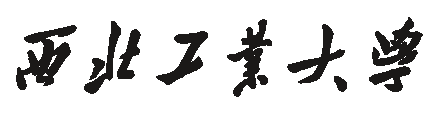
\includegraphics[scale=1.5]{pic/university_text_logo}\\
		\vspace{9pt}
		\sXiaoyi 研究生课程考试答题册
	\end{center}
	
	% 连续三个四号的空格 14.4*3
	\vspace{43.2pt}
	
	% 得分表
	% 宽4.3 高1.92
	
	
	\begin{table}[h]
		%	\renewcommand\arraystretch{2}
		\begin{tabular}{p{8cm}|p{44mm}|}
			\cline{2-2}
			& \vspace{6pt}
			\sSihao \fKai 得分: 
			\vspace{12pt}
			\\ \cline{2-2}
			
		\end{tabular}
	\end{table}
	
	% 小四空格
	\vspace{14.4pt}
	
	% 填空
	\begin{center}
		\vskip 2cm
		{
			\sSihao 学~~~~~~号 \coverunderline[5.5cm]{}\\
			\vskip 0.7cm
			\sSihao 姓~~~~~~名 \coverunderline[5.5cm]{}\\
			\vskip 0.7cm
			\sSihao 考试课程 \coverunderline[5.5cm]{几何造型原理和应用}\\
			\vskip 0.7cm
			\sSihao 考试时间 \coverunderline[5.5cm]{2017年12月30日}
			%\vfill
		}
	\end{center}
\end{titlepage}